\documentclass[a4paper, gray]{beamer}

\usepackage{times}

\usepackage{verbatim}
\usepackage{color}
\usepackage{listings}

\usepackage{xcolor}
\definecolor{ocre}{RGB}{243,102,25}

\usepackage[german]{babel}
\usepackage[utf8]{inputenc}
\usepackage[T1]{fontenc}

\usepackage{multicol}

%\usepackage{exercise}

\usepackage{graphicx}

\usetheme{default}

%\usepackage{pgfpages}
%\pgfpagesuselayout{resize to}[a4paper,landscape]

\logo{\pgfimage[width=1cm,height=1cm]{img/fhnw_logo}}

\definecolor{lbcolor}{rgb}{0.92,0.92,0.92}
\definecolor{cmtcolor}{rgb}{0.0,0.5,0.0}
\lstset{numbers=left,
        numberstyle=\tiny,
        keywordstyle=\color{blue}\bfseries\sffamily,
        identifierstyle=\ttfamily,
        commentstyle=\em,
        stringstyle=\ttfamily,
        extendedchars=true,
        showstringspaces=false,
        language=c++,
        backgroundcolor=\color{lbcolor},
        commentstyle=\color{cmtcolor}}

\RequirePackage[framemethod=default]{mdframed}

% Exercise box	  
\newmdenv[skipabove=7pt,
skipbelow=7pt,
rightline=false,
leftline=true,
topline=false,
bottomline=false,
backgroundcolor=ocre!10,
linecolor=ocre,
innerleftmargin=5pt,
innerrightmargin=5pt,
innertopmargin=5pt,
innerbottommargin=5pt,
leftmargin=0cm,
rightmargin=0cm,
linewidth=4pt]{eBox}

% Theorem box
\newmdenv[skipabove=7pt,
skipbelow=7pt,
backgroundcolor=black!5,
linecolor=ocre,
innerleftmargin=5pt,
innerrightmargin=5pt,
innertopmargin=5pt,
leftmargin=0cm,
rightmargin=0cm,
innerbottommargin=5pt]{tBox}



\newcounter{dummy} 
\numberwithin{dummy}{section}

\newtheorem{exerciseT}{Exercise}[section]
%\newtheorem{theoremeT}[dummy]{Theorem}
%\newtheorem{exampleT}{Example}[section]

\newenvironment{exercise}{\begin{eBox}}{\hfill{\color{ocre}\tiny\ensuremath{\blacksquare}}\end{eBox}}
%\newenvironment{exercise}{\begin{eBox}\begin{exerciseT}}{\hfill{\color{ocre}\tiny\ensuremath{\blacksquare}}\end{exerciseT}\end{eBox}}
%\newenvironment{theorem}{\begin{tBox}\begin{theoremeT}}{\end{theoremeT}\end{tBox}}
%\newenvironment{example}{\begin{exampleT}}{\hfill{\tiny\ensuremath{\blacksquare}}\end{exampleT}}


\title{AI Programming with Python}
\subtitle{FHNW Medical Informatics}
\author{Dave Herzig}
%\institute{scifortek.com}
\date{\today}

\begin{document}

\frame{\titlepage}

\setcounter{tocdepth}{1}

\frame
{
	\frametitle{Agenda}
	\small {\tableofcontents}
}

\section{Programming Environment}

\begin{frame}[fragile]
  \frametitle{Jupyter Notebook}
  Everyone should use the same programming environment. As we do not want to waste time with
  installing software, we use Google Colab.\\
  \verb|https://colab.research.google.com|\\
  \vspace{3mm}
  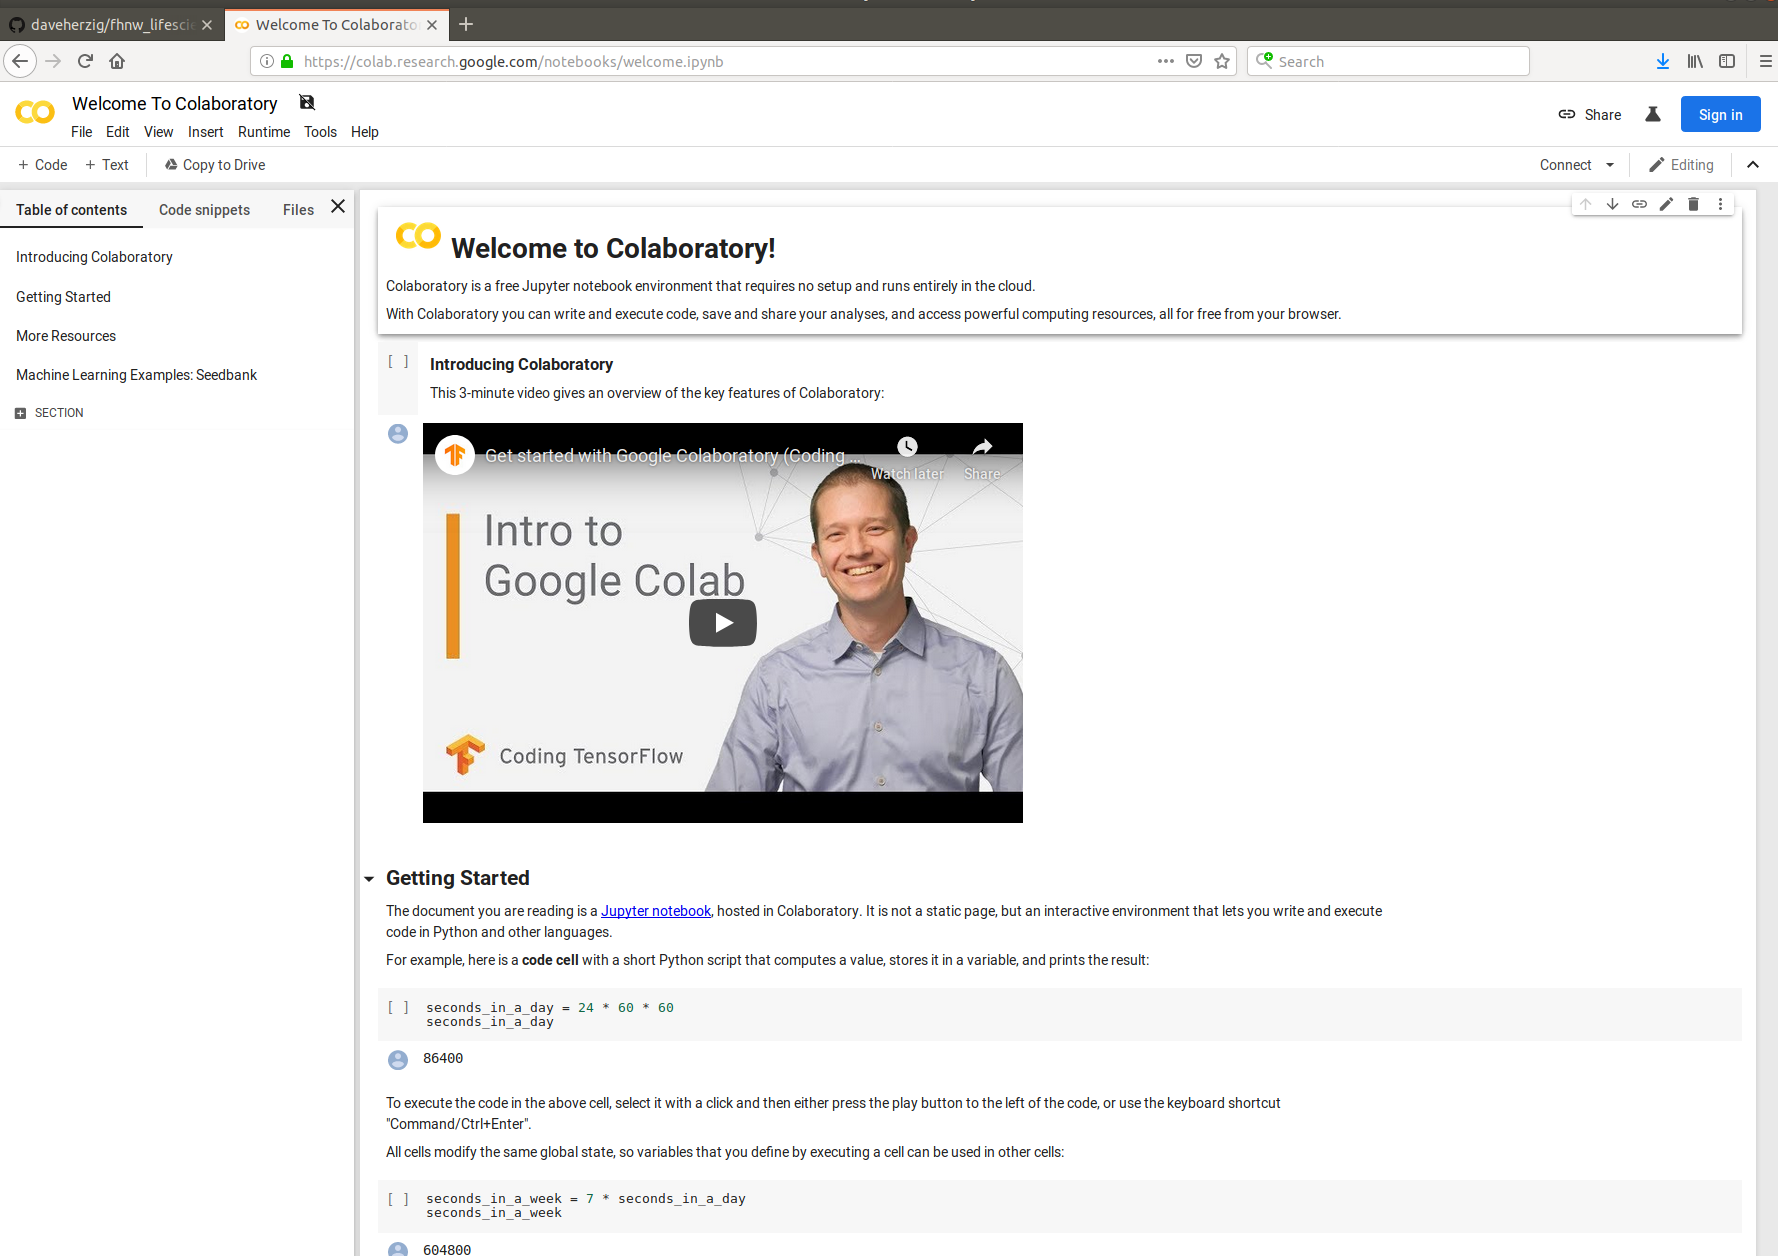
\includegraphics[scale=0.1]{img/jupyter_notebook}
\end{frame}


\begin{frame}[fragile]
  \frametitle{Python Frameworks}
  The following python frameworks will be used:
  \begin{itemize}
  \item Numpy
  \item Pandas
  \item Tensorflow
  \end{itemize}
\end{frame}

\begin{frame}[fragile]
  \frametitle{Jupyter Notebook}
  \begin{exercise}
  Write (and run) your first Jupyter notebook on Google Colab!
  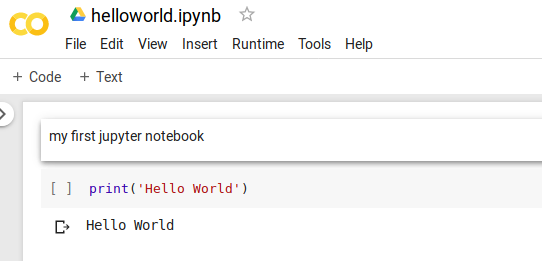
\includegraphics[scale=0.5]{img/jupyter_notebook_exercise}
  \end{exercise}
\end{frame}

\section{Basics}

\begin{frame}[fragile]
  \frametitle{Jupyter Notebook}
  Everyone should use the same programming environment. As we do not want to waste time with
  installing software, we use Google Colab.\\
  \verb|https://colab.research.google.com|
  
\end{frame}


\begin{frame}[fragile]
  \frametitle{Python Frameworks}
  The following python frameworks will be used:
  \begin{itemize}
  \item Numpy
  \item Pandas
  \item Tensorflow
  \end{itemize}
\end{frame}

%\include{memory}

%\include{commandline}
%\include{oop}
%\include{inheritance}
%\include{ruleofthree}
%\include{template}
%\include{stl}
%\include{ad}
%\include{recursion}
%\include{sorting}
%\include{searching}
%\include{datastructures}
%\include{tree}
%\include{graph}
%\include{stringmatching}
%\include{qt}

%\include{samples}

\end{document}
